\documentclass[11pt,compress,t,notes=noshow, aspectratio=169, xcolor=table]{beamer}

\usepackage{../../style/lmu-lecture}
% Defines macros and environments
% This file is included in slides and exercises

% Rarely used fontstyle for R packages, used only in 
% - forests/slides-forests-benchmark.tex
% - exercises/single-exercises/methods_l_1.Rnw
% - slides/cart/attic/slides_extra_trees.Rnw
\newcommand{\pkg}[1]{{\fontseries{b}\selectfont #1}}

% Spacing helpers, used often (mostly in exercises for \dlz)
\newcommand{\lz}{\vspace{0.5cm}} % vertical space (used often in slides)
\newcommand{\dlz}{\vspace{1cm}}  % double vertical space (used often in exercises, never in slides)
\newcommand{\oneliner}[1] % Oneliner for important statements, used e.g. in iml, algods
{\begin{block}{}\begin{center}\begin{Large}#1\end{Large}\end{center}\end{block}}

% Don't know if this is used or needed, remove?
% textcolor that works in mathmode
% https://tex.stackexchange.com/a/261480
% Used e.g. in forests/slides-forests-bagging.tex
% [...] \textcolor{blue}{\tfrac{1}{M}\sum^M_{m} [...]
% \makeatletter
% \renewcommand*{\@textcolor}[3]{%
%   \protect\leavevmode
%   \begingroup
%     \color#1{#2}#3%
%   \endgroup
% }
% \makeatother


%\title{iML: Ante-hoc Methods for Neural Networks}
%\subtitle{Instance-wise Feature Selection}
\title{Interpretable Machine Learning}
\date{}

\begin{document}
	%\maketitle
	\graphicspath{ {./figure/} }

\newcommand{\titlefigure}{figure/bild9}
\newcommand{\learninggoals}{
\item Instance-wise feature selection
\item Explain then predict models
\item Optimizing using explanation data}

\lecturechapter{Instance-wise Feature Selection}
\lecture{Interpretable Machine Learning}

 
\begin{frame}{Instance-wise Feature Selection}
\begin{itemize}
    \item Select a subset of features conditioned or based on the input instance
    \begin{itemize}
        \item Two instances might not have the same feature mask
    \end{itemize}
    \bigskip
    \item Instance-wise feature selection similar to feature attribution — important features are
selected
\item Unambiguous with respect to explanation (more on that later)
\end{itemize}
    
\end{frame}

\begin{frame}{Instance-wise Feature Selection - Example in Language}


\centerline{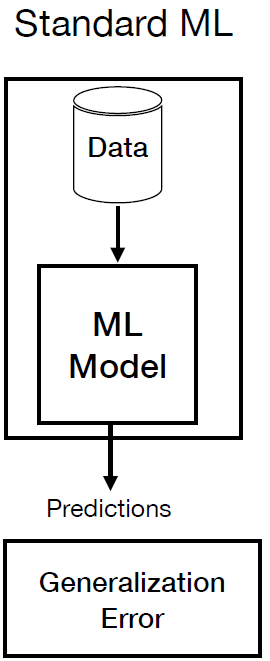
\includegraphics[width=0.15\linewidth,left]{bild5}}

\end{frame}

\begin{frame}{Instance-wise Feature Selection - Example in Language}

\centerline{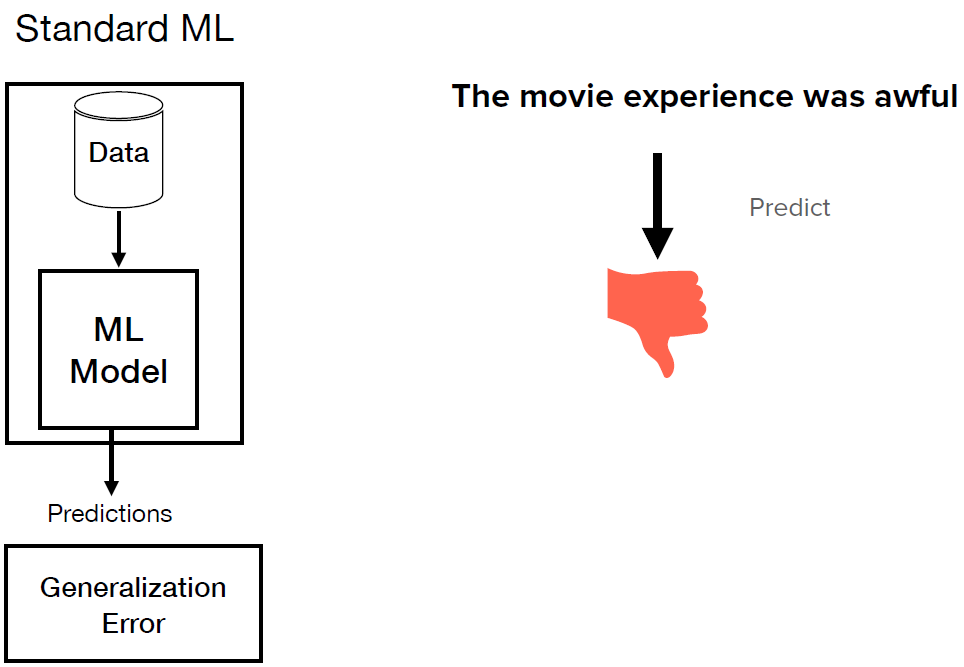
\includegraphics[width=0.6\linewidth,left]{bild6}}

\end{frame}

\begin{frame}{Instance-wise Feature Selection - Example in Language}
    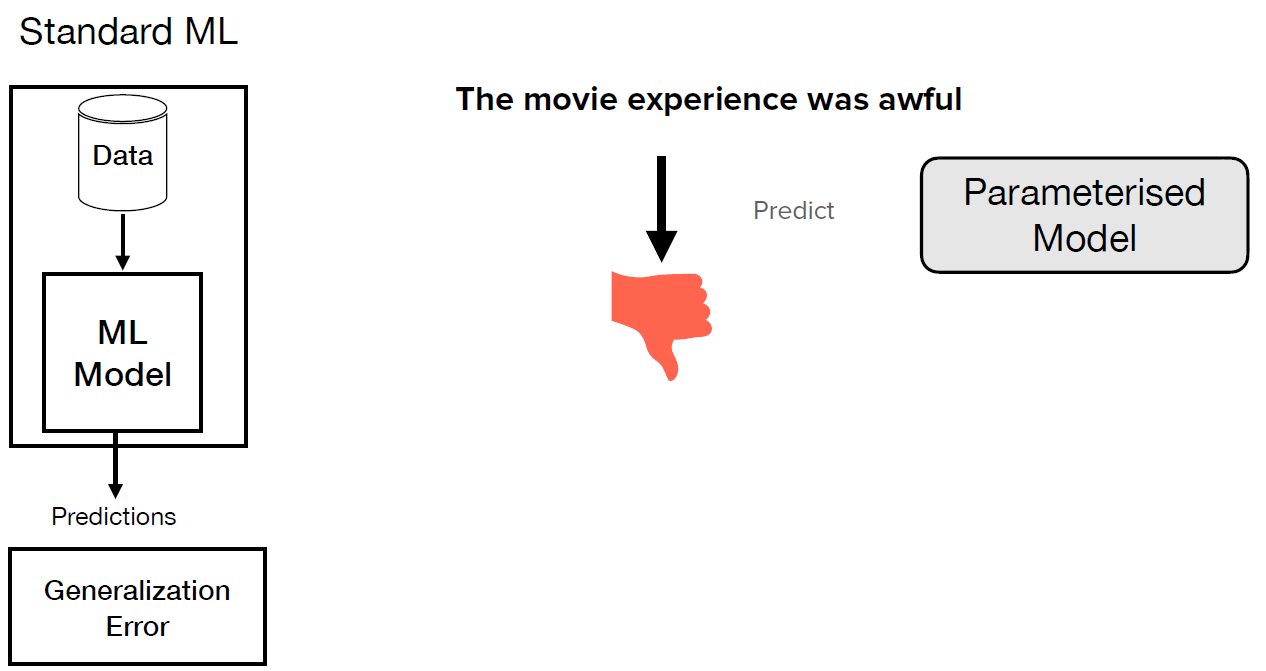
\includegraphics[scale=.36, left]{bild7}
\end{frame}

\begin{frame}{Instance-wise Feature Selection - Example in Language}


    \begin{figure}
    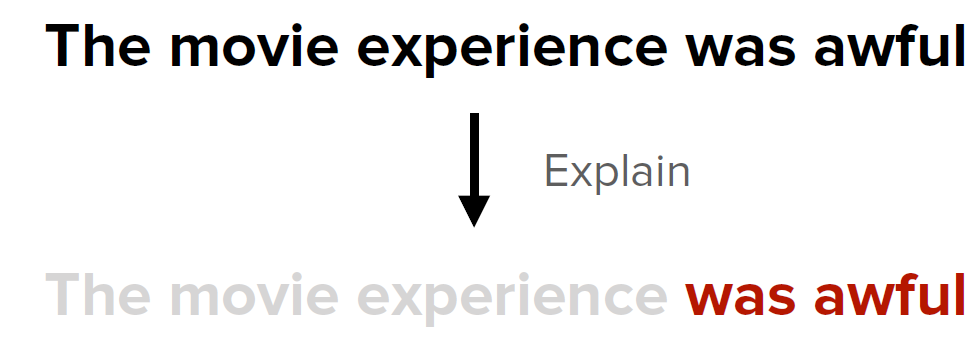
\includegraphics[width=0.6\linewidth]{bild8}
    \end{figure}
\end{frame}

\begin{frame}{Instance-wise Feature Selection - Example in Language}
    \begin{figure}
    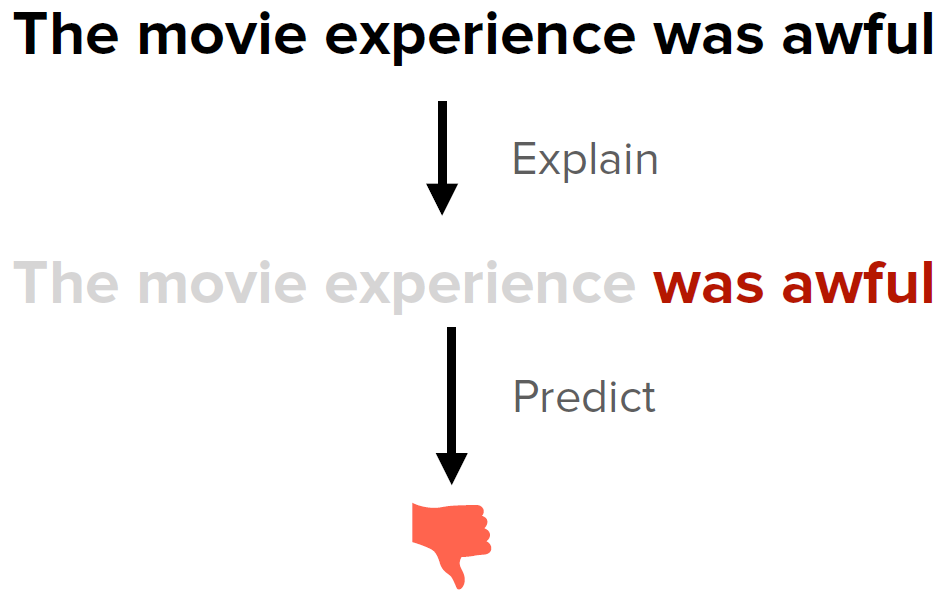
\includegraphics[width=0.6\linewidth]{bild9}
    \end{figure}
\end{frame}

\begin{frame}{Instance-wise Feature Selection - Example in Language}
    \begin{figure}
    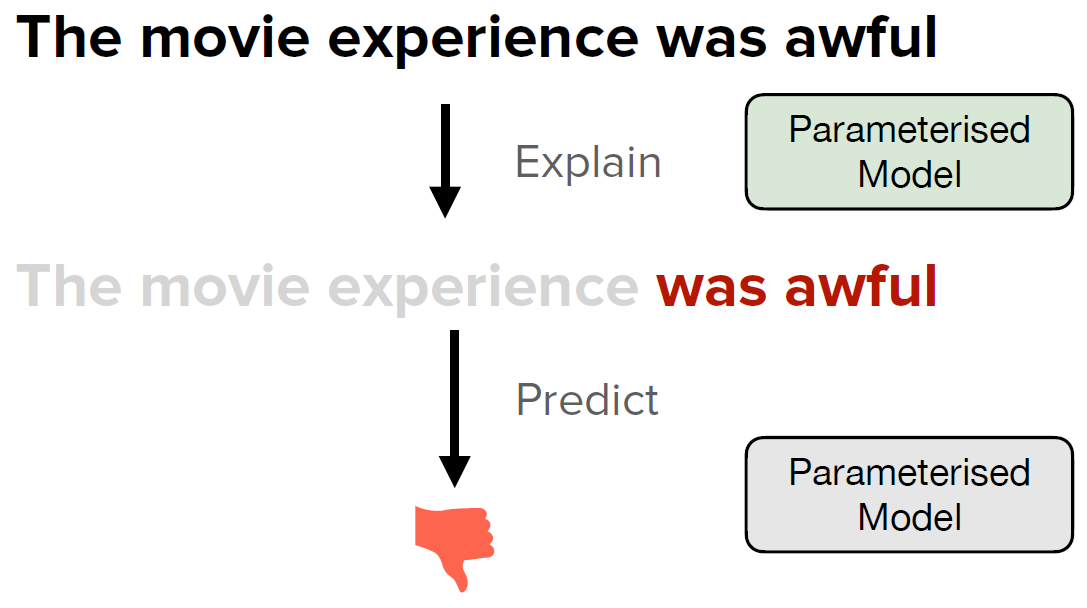
\includegraphics[width=0.6\linewidth]{bild10}
    \end{figure}
\end{frame}

\begin{frame}{Instance-wise Feature Selection - Example in Language}
    \begin{figure}
    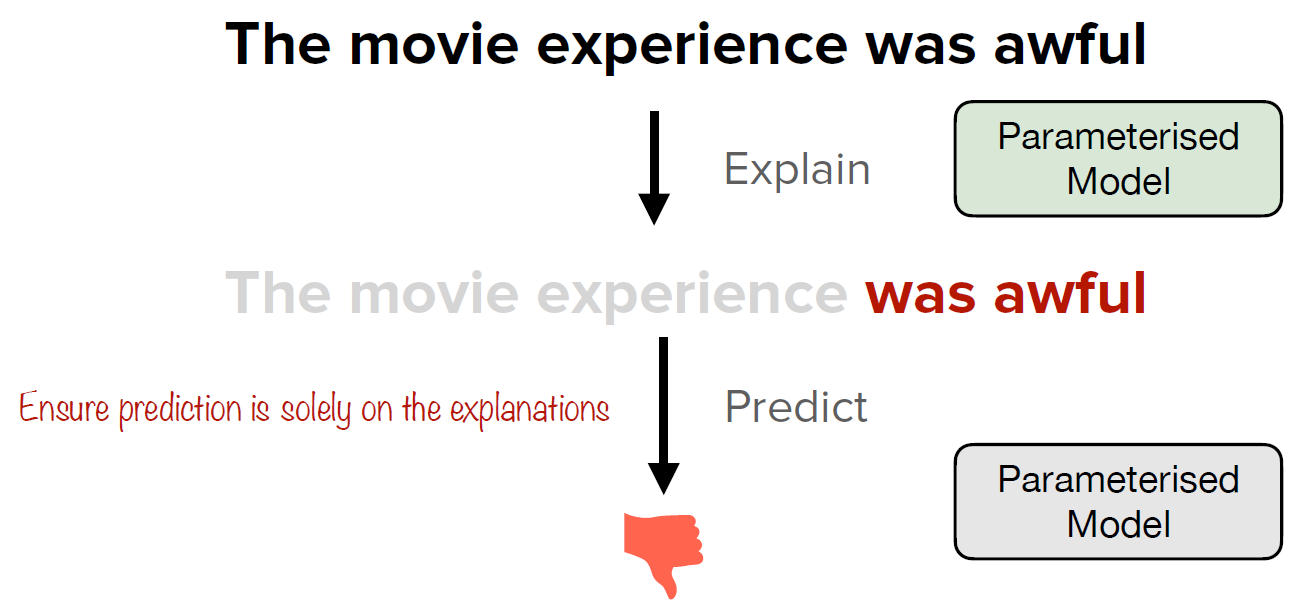
\includegraphics[width=0.6\linewidth]{bild11}
    \end{figure}
\end{frame}

\begin{frame}{Instance-wise Feature Selection - Example in Language}
    \begin{figure}
    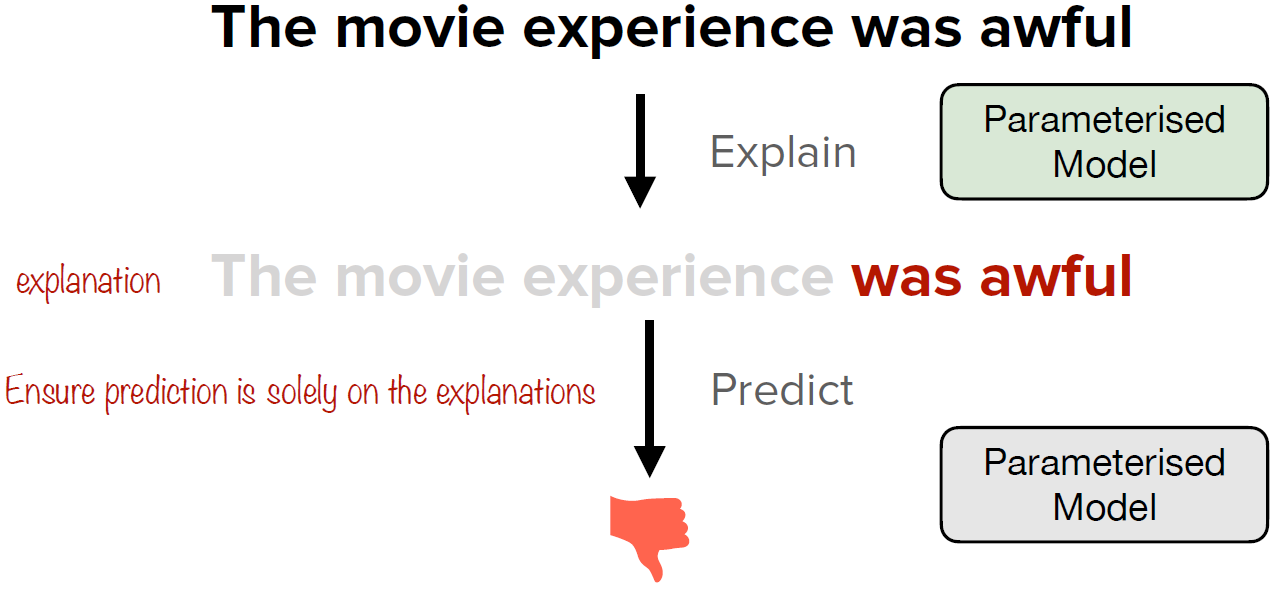
\includegraphics[width=0.6\linewidth]{bild12}
    \end{figure}
\end{frame}

\begin{frame}{Explanation Data}
    \begin{figure}
    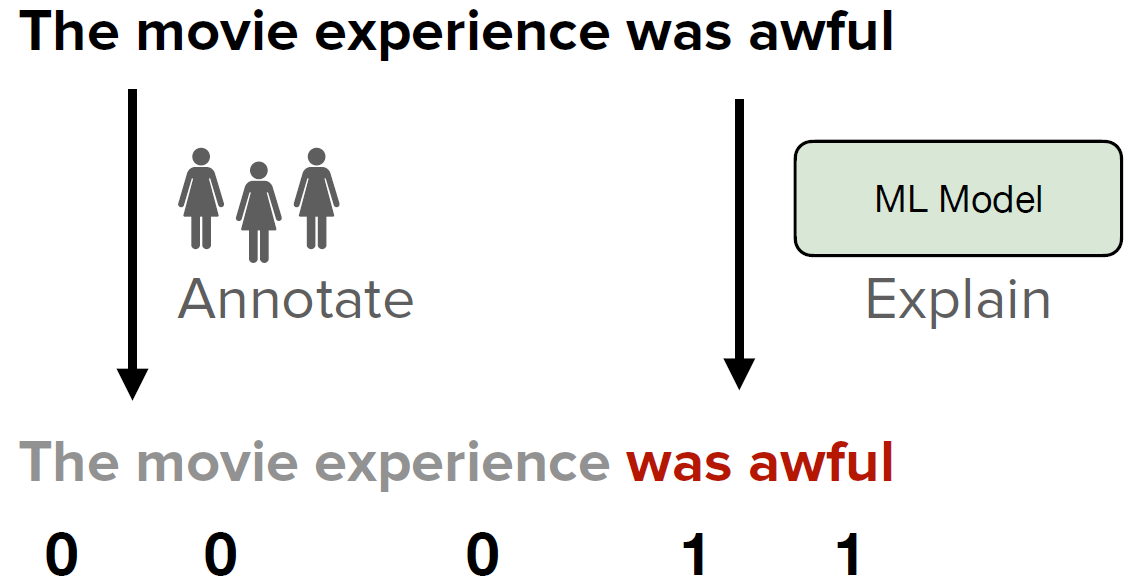
\includegraphics[width=0.6\linewidth]{bild13}
    \end{figure}
\end{frame}

\begin{frame}{Explanation Data}
    \begin{figure}
    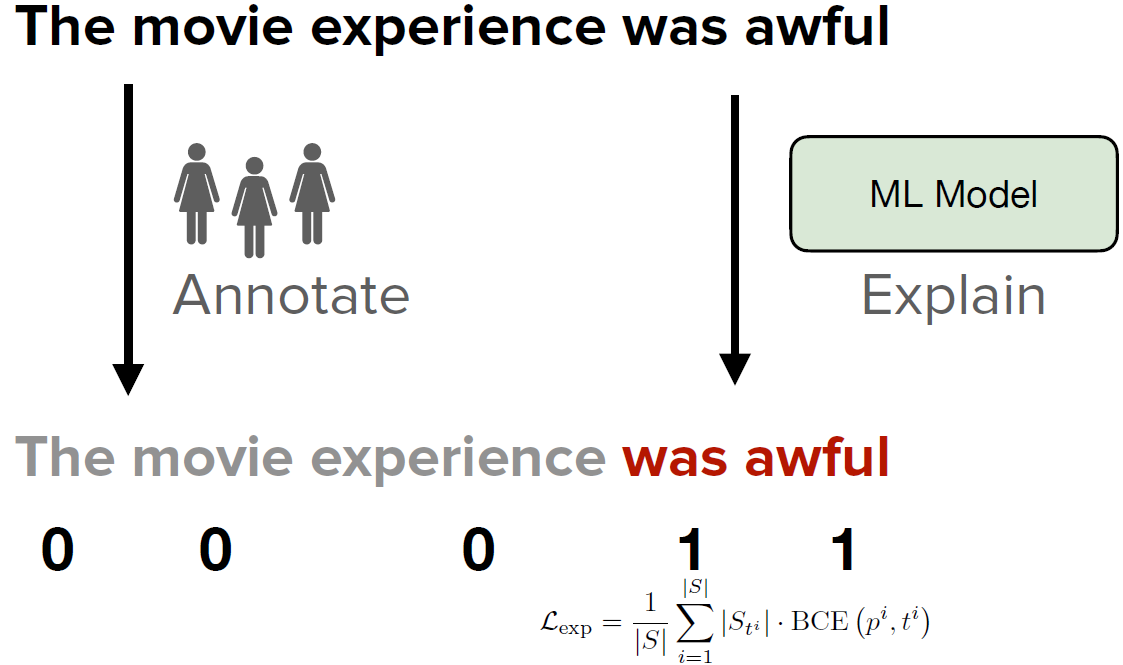
\includegraphics[width=0.6\linewidth]{bild14}
    \end{figure}
\end{frame}


\begin{frame}{Explanation Data}
    \begin{figure}
    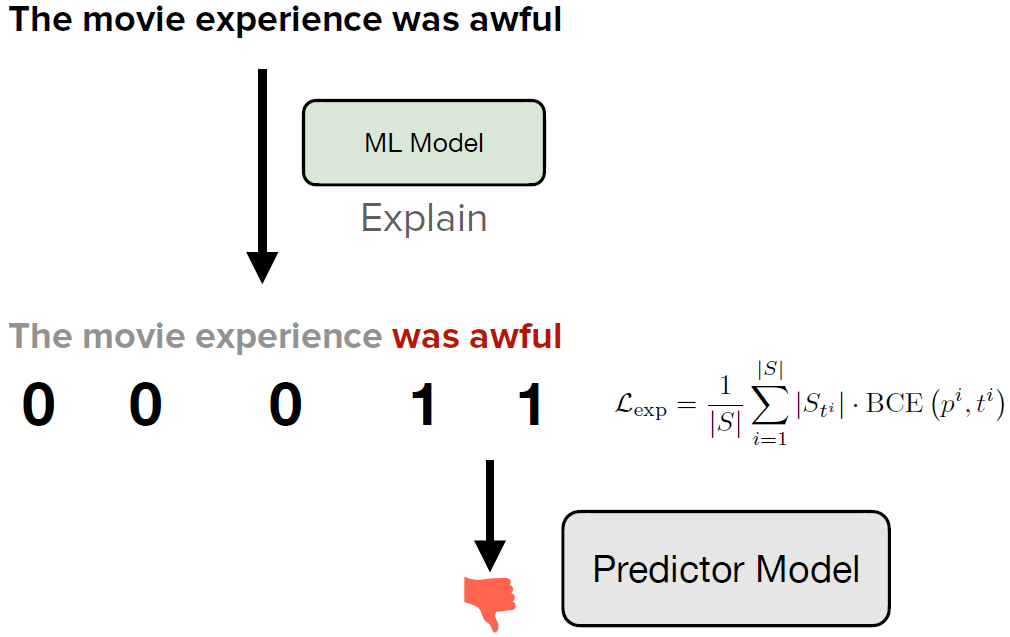
\includegraphics[width=0.7\linewidth]{bild15}
    \end{figure}
\end{frame}

\begin{frame}{Explain then Predict using Explanation data}
\begin{itemize}
    \item Selecting features conditioned on individual instances results in better task performance in
comparison to global feature selection
    \bigskip
    \item Instance-wise feature selection has higher inherent sparsity
    \bigskip
    \item The output of the feature-selection stage is the explanation
    \bigskip
    \item The predictor depends solely on the masked input and therefore unambiguous with respect to
explanation
\end{itemize}
    
\end{frame}



\endlecture
\end{document}